\lecture{10}{2025-03-19}{Encryption?}{}
\begin{parag}{Exercice}
    Determine the minimum average length of the binary key for a cryptosystem that has the following characteristics
\begin{itemize}
    \item the message is an uncompressible binary string of length $n$
    \item the system achieves perfect secrecy
\end{itemize}
\begin{subparag}{Solution}
    \begin{itemize}
        \item $H(T)$ must be essentially $n$ bits (otherwise further compression is possible
        \item Perfect secrecy requires $H(T) \leq H(K)$
        \item  hence $H(K)$ is at least $n$
        \item The average blocklength of the binary key is at least $n$ bits
    \end{itemize}
\end{subparag}
\end{parag}

\begin{parag}{Symettric-Key crypto Systems: key-distribution problem}
         A symmetric-key cryptosystem is one for which both ends use the same key $(k_A = k_B=k)$. All example considered so fare rely on a symmetric key\\
         There exists fast (ans secure) symmetric key cryptosystems, but:
         \begin{itemize}
             \item Anybody that has the key can encrypt and/or decrypt
             \item The key cannot be sent over an insecure channel
             \item In an $n$ user network, each user needs $n-1$ keys to communicate privately with every other user. Key distribution is a problem as it hat to be done over a secure channel. And keys have to be changed frequently
             \item We have a real problem (the first $6$min. and $20$ secs of:
                 \begin{center}
                 \url{https://www.youtube.com/watch?v=YEBfamv-_do}
                 \end{center}
                 
                 
         \end{itemize}
         However, is there a way to distribute keys over a pubic channel?
\end{parag}
\begin{parag}{Solution}
    In 1976, Diffie and Hellman came up with a solution.
    \begin{subparag}{Example}
        You pick a number $p = 7$ which is a prime $ \mathcal{A} = \{0, 1,2 , 3, 4, 5, 6\}$. We then take $ g = 3$
        \begin{center}
           
        \begin{tabular}{cc}
            $i$ & $g^i \mod 7$ \\
            0  & \\
            1 & 3 \\
            2 & 2\\
            3 & 6\\
            4 & 4\\
            5 & 5\\
            6 & 1
        \end{tabular}
        \end{center}
        The gives us a permutation. We have to be careful with choosing the $g$ because for example if we take $g = 2$, and take $g^1$ and $g^4$ the result is $2$ which leads that we don't have a permutations
        
    \end{subparag}
How does it is seen:
\begin{center}
    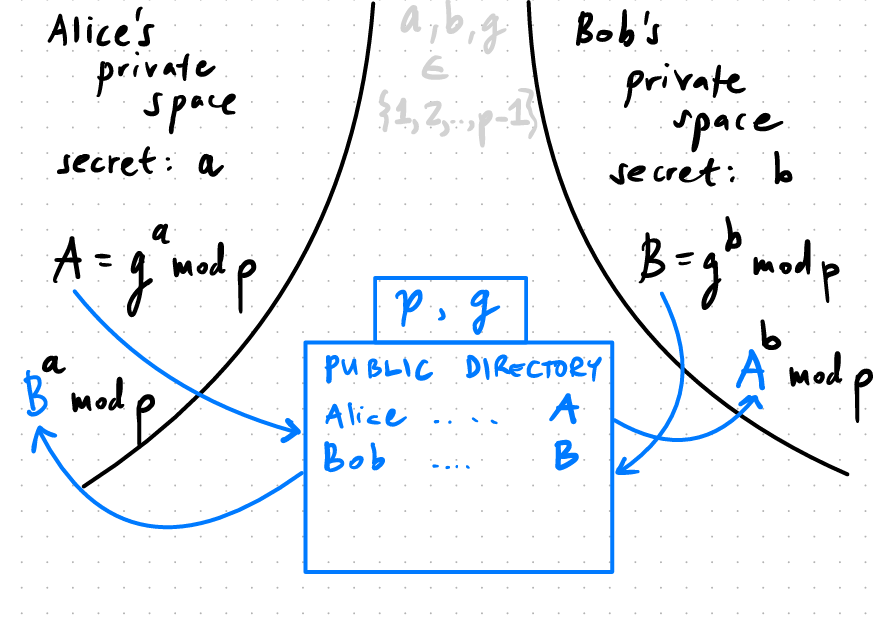
\includegraphics[scale=0.4]{12025-03-19.png}
\end{center}
We have a public directory like a phone book where everyone has access. Alice pick a random $a$. Then she takes a public $A = g^a \mod p$ which we will be written in the public directory. Then Bob do the same thing.  \\
When Alice and Bob want to have an interaction. Alice will look for Bob in the phonebook, take the $B$ in her private space, take the result of $B^a \mod p$ (she is the only one to know $a$). Bob do the same thing: $A^b \mod p$\\
\textbf{At this point} 
\begin{itemize}
    \item Alice has  $B^a \mod p$
        \begin{align*}
            B^a = (g^b \mod p)^a \mod p
        \end{align*}
    \item Bob has $A^b \mod p$
        \begin{align*}
            A^b = (g^a \mod p)^b \mod p
        \end{align*}
        
        
       
\end{itemize}
\begin{subparag}{Fact}
    \begin{theoreme}
        For all $x, y, m \in \mathbb{Z}$:
        \begin{align*}
            \left[ (x \mod m) \cdot (y \mod m) \right] \mod m = xy \mod m
        \end{align*}
        
    \end{theoreme}
    We then get $B^a = g^{ab} \mod p$ and $A^b = g^{ab} \mod p$ We juste need to find the inverse of $g^i \mod p$ Which is a discrete logarithm problem. It is very hard to find the discrete logarithm. The gives the secrecy of this encryption. The secrecy is only here because it is hard to compute this inverse

\end{subparag}
\begin{subparag}{Secrecy}
    But can't anybody generate this key?\\
    We all know $g$ and we know that $A = g^a \mod p$ we juste has to find
    
\end{subparag}
\begin{subparag}{Eve wants to listen}
    Assuming that the cryptosystem used by Bob and Alise is secure, the best option for Eve is to find the key $k$. \\
    She know $p, g, A$ and $B$.\\
    In generale, there seems to be no better way than finding the number $a$ for which $g^a = A$, and the comput $k = B^a$\\
    This is a problem. Let us check out some number. Suppose $p$ is a 2048 bit number. (it must be prime, but let us neglect this and assume $p  = 2^{2048}$ How long does it take to compute:
    \begin{align*}
        2\log_2 p = 4096
    \end{align*}
    Multiplications to performs $a \to g^a$ (called discrete exponentiation). With a computer that performs $10^{10}$ multiplications per seconds, the exponentiation is done seamlessly.\\
    It takes roughly:
    \begin{align*}
        \text{exp} \left( \left( \frac{64}{9} \right)^{ \frac{1}{3}} (\ln p)^{ \frac{1}{3}} \ln \ln p)^{ \frac{2}{3}} \right) \approx 10^{35}
    \end{align*}
    Mutliplication to perform $g^a \to a$ (called discrete logarithm to the base $g$. With the same computer, it takes about $10^{25}$ seconds, which is about $7 \cdot 10^{7}$ times the ages of the earth.
\end{subparag}
\begin{subparag}{Conclusion}
    Diffie and Hellman's public key distribution scheme is clever, efficient, and it seems to be secure.
\end{subparag}
\end{parag}

\begin{parag}{Paradigm shift}
    The issue with the security is the computation. For example in maybe a couple of years the quantum computer will be able to compute this discrete algorithm very fast. The DG system would instanlty become insecure.\\
    To the constrast, perfect secrecy offers provable security even when the enemy has infinite time and computing power. Most cryptographic systems rely on computational security


\end{parag}
\begin{parag}{One way function}
    Discrete exponentiation is an example of a one  way function: a function for which a fast algorithm exists one way but not in the other way. The case for the discrete logarithm is that there is a way back but it is very slow. However, the best case would be that there is not way back.
    \begin{subparag}{Example}
        IF a computer were to save user's names and passwords, a sstem manager would have access to both.\\
        This is not the case if the operating system stores, along the name a one-way function $f$ of our password.( The password itself is never stored)
        
    \end{subparag}
    
\end{parag}

\begin{parag}{Trapdoor One-way function}
    A tropdoor one way function is a one-way function with an extra feature called the trapdoor information: with this information, the hard-to-carry out inverse computation becomes easy.\\
    Diffie and Hellmann realized that with such a tool the key distribution problem would diseappear

\end{parag}



\begin{parag}{Asymetric cryptography}
    Suppose that Allice wants to send private information to Bob\\
        Bob has a trapdoor one-way function, implemented by an algorithm $E_B$ that he publsishes in a open directory\\
        He is the only one who has the trapdoor information $k_B$. Hence he has the algorithm $D_B$ that implements the inverse function.\\
        Alice and Bob no longer need a shared key:
        \begin{center}
           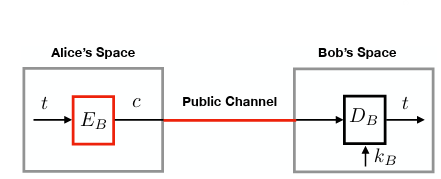
\includegraphics[scale=0.8]{22025-03-19.png} 
        \end{center}

\end{parag}
\begin{parag}{ElGammal's trapdoor one way function}
    \begin{subparag}{Setup}
        \begin{itemize}
            \item Fix a large prime number $p$. Hereafter all the numbers are in $\{0, 1, \dots, p1\}$ and arithmetic is modulo $p$ (mor on it later).
            \item Pick a generator $g$
            \item Pick randomly selected numbers $x$ and $y$. Unlike $p$ and $g$,$x$, and $y$ are kept secret.\\
            \item  Here is a trapdoor one-way function, with \important{trapdoor information} $x$.
                \begin{center}
                    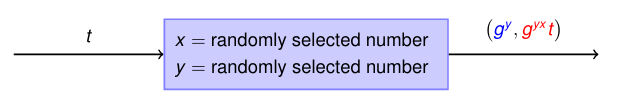
\includegraphics[scale=0.5]{32025-03-19.png}
                \end{center}
        \end{itemize}
        
        Given the trapdoor information $x$, we can invert the function as follows:
        Compute the inverse of $g(^y)^x = g^{xy}$, multiply the result with $g^{xy}t$. The result is $t$.
    \end{subparag}
\begin{subparag}{More concretly}
    Alice has:
    \begin{itemize}
        \item $t$ = plaintex, $t$
        \item $y = $ random number, $y$
    \end{itemize}
    Bob:
    \begin{itemize}
        \item $x$ = random number $x$.
    \end{itemize}
    The scheme look like this:
    \begin{center}
        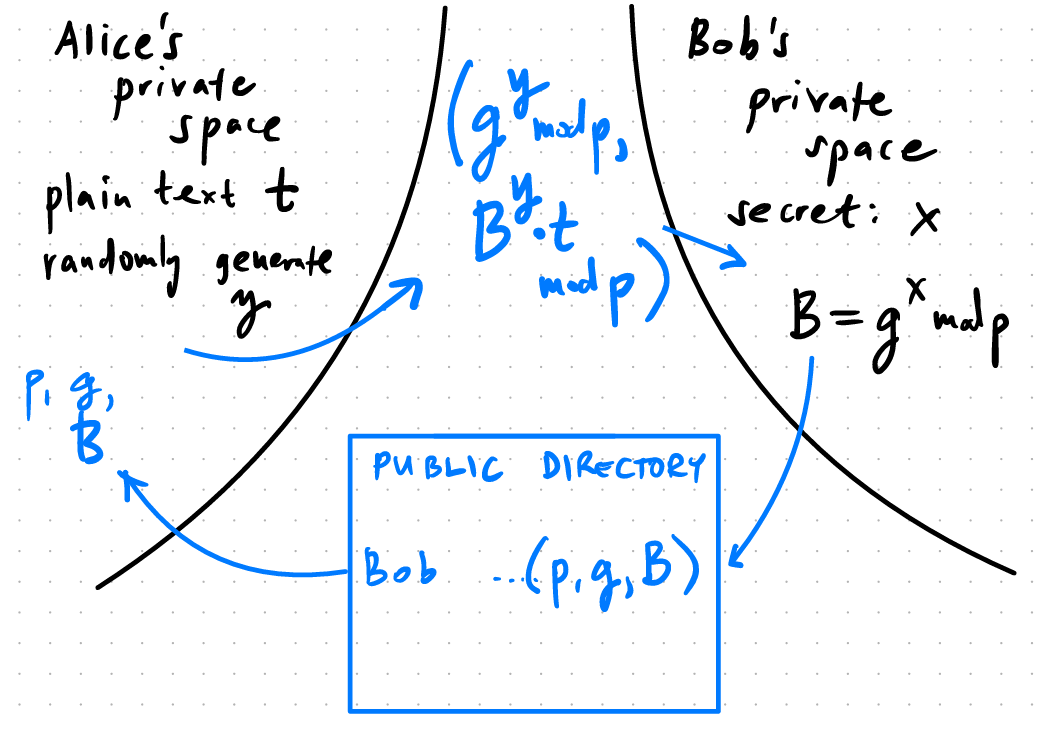
\includegraphics[scale=0.5]{42025-03-19.png}
    \end{center}
    Bob sends $g^x$ to Alice, then Alice sends the cryptogram $(g^y, g^{xy}t)$ to Bob
    \begin{framedremark}
        Note: $x$ and $y$ are transaction specific
    \end{framedremark}
    
    
    
    
\end{subparag}
\end{parag}

